% -----------------------------------------------------------------------
% -----------------------------------------------------------------------
% -----------------------------------------------------------------------
% Einleitung
% -----------------------------------------------------------------------
% -----------------------------------------------------------------------
% -----------------------------------------------------------------------
\chapter{Introduction}

\section{Motivation: An Open-Domain Comparative Argumentative Machine (CAM)}

%
%The topic of this master thesis is \emph{Argument Mining}, more precisely \emph{Comparative Argument Mining}. Argument Mining is an area in Natural Language Processing which gained popularity quite recently. The first workshop organized by the \emph{Association for Computational Linguistics} (ACL) was just hold three years ago, in 2014 (\cite{W14-21:2014}).\\
%The aim of Argument Mining is the analysis of arguments in natural language. One can identify three main tasks: the identification of argumentative sentences, the components of an argument and their relations (cite). There are several definitions of the term \emph{argument} and it's structure (see section \ref{sec:argth}). In Argument Mining, the Claim/Premise model is often used. A claim is the statement of a sentence which is supported or attacked by one or more premises. An argument of this structure may look like the following:
%\begin{quote}
%    [X will win$]_{claim}$ [because$]_{support}$ [X can do Y$]_{premise}$
%\end{quote}
%The knowledge obtained by analyzing such sentences can be used \ldots\newline
%
%Comparative Arguments are a special kind of arguments. The claim of a comparative argument is a comparison between one or more objects. The comparison frequently contains a direction (or polarity) in a sense that \emph{A is better / worse than B}.
%



\chapter{Background}
\section{Related Work}
\label{sec:argth}
\label{sec:argmine}
\cite{Lippi2016Argumentation-M} gave a summary of the research topic \emph{Argument Mining} in general. They introduced five dimensions to describe argument mining problems: granularity of input, the genre of input, argument model, the granularity of target and goal of analysis.  Furthermore, the typical steps of argument mining systems are defined. First, the input must be divided into argumentative (e.g. claim and premise) and non-argumentative parts. This step is described as a classification problem. Second, the boundaries of the argumentative units must be identified; this is understood as a segmentation problem. Third, the relations between argumentative units must be identified. For instance, claims and premises might be connected with a \emph{support} or a \emph{attack} relation.


%07 biomed


A system which is capable of recognising comparative sentences and their components such as the compared entities, the property on which the entities are compared to and the direction of comparison was presented in \cite{fiszman2007interpreting}. The evaluation showed that the outcome has a high quality (f1 score of 0.81). However, the presented system is specific to the domain of studies to drug therapy. The system uses patterns generated from sentences, as well as domain knowledge. Therefore, the methods cannot easily be transferred for the problem of this thesis.

%  12 sci
\cite{park2012identifying} presented a domain-specific approach on argumentative sentence detection. The problem is formulated as a binary classification task (a sentence is either comparative or not). As in \cite{fiszman2007interpreting}, the features are tailored for medical publications. Lexical features capture the presence of specific words, many of them bound to the medical domain. The analysis of 274 sentences resulted in syntactic features. Similar to \cite{fiszman2007interpreting}, the features cannot be directly transferred to other domains.

% 10 biomed
A recent publication on \emph{Comparative Argument Mining} is \cite{gupta2017identifying}, where a set of rules for the identification of comparative sentences (and the compared entities) is derived from \emph{Syntactic Parse Trees}. With those rules, the authors achieved a F1 score of 0.87 for the identification of comparative sentences. The rules were obtained from 50 abstracts of biomedical papers. Such being the case, they are domain dependent.\newline

Because this thesis deals with user-generated content from the web, publications dealing with similar data are of interest.

The challenges occurring while processing texts from social media are described in \cite{Snajder2017Social-Media-Ar}.  In this publication, social media is broadly defined as \enquote{less controlled communication environments [...]}. Besides the noisiness of text, missing argument structures and poorly formulated claims are mentioned. It is expected that the text used in this thesis will have the same shortcomings. Additionally, \cite{Snajder2017Social-Media-Ar} emphasized that analyzing social media texts can delivery reasons behind opinions. 

In addition to the challenges mentioned above, \cite{Dusmanu2017Argument-Mining} also points to the specialized jargon in user-generated content like hashtags and emoticons. With this in mind, \cite{Dusmanu2017Argument-Mining} classified tweets about the \enquote{Brexit} and \enquote{Grexit} either as argumentative or as non-argumentative. Besides features used in other mentioned papers, new features covering hashtags and sentiment are added. They achieved a F1 score of 0.78 (using Logistic Regression) for the classification. It must to be said that the data set is small (1887 tweets) and the domain is rather specific.\newline

Many publications on argument mining are dealing with a classification problem of some kind. Publications dealing with the identification of argument structures are of relevance for this thesis, as they provide valuable insights on the suitability of features and algorithms.

%what works and what does not
\cite{Aker2017What-works-and-} summarized and compared features used in other publications for identification of argumentative sentences. In addition, a Convolutional Neural Network (as described in \cite{Kim2014Convolutional-N}) was tested. Two existing corpora and six different classification algorithms were used. As a result, structural features are most expressive; Random Forest is the best classifier.

\cite{Stab2014Identifying-Arg} described a two-step procedure to identify components of arguments (such as claim and premise) and their relationships (like \enquote{premise A supports claim B}). The identification step is formulated as a multi-class classification. For the identification of argumentative components, a F1 score of 0.72 is reported.

%essence of a claim
How different datasets represent the argumentative unit of a \emph{claim} is analysed in \cite{Daxenberger2017What-is-the-Ess}. After an analysis of the datasets and their annotation scheme, \cite{Daxenberger2017What-is-the-Ess} conducted two experiments.
In the first one, each learner (Logistic Regression, Convolutional Neural Networks and LSTM) was trained and evaluated (10-fold cross-validation) on each dataset one after another. On average, the macro F1 score for identifying claims was 0.67 (all results ranging from 0.60 to 0.80). No significant difference between the results of Logistic Regression and the neural models was found. In isolation, lexical features, syntactical features and word embeddings were most helpful. Structural features turned out to be the weakest.
The second experiment was conducted in a cross-domain fashion. For each pair of datasets, one was used as the training set and the other one as the test set. The average macro F1 score was 0.54. In this scenario, the best feature combination outperformed all neural models. However, it is assumed that there might not be enough training data for the neural models.
As the last point, \cite{Daxenberger2017What-is-the-Ess} noted that all claims share at least some lexical clues.


The role of discourse markers in the identification of claims and premises are discussed in \cite{Eckle-Kohler2015On-the-Role-of-}. A discourse marker is a word or a phrase which connects discourse units. For instance, the word \enquote{as} can show a relation between claim and premise: \enquote{As the students get frustrated, their performance generally does not improve}.  A similar function for words like \enquote{better}, \enquote{worse} or \enquote{because} is expected in this thesis. \cite{Eckle-Kohler2015On-the-Role-of-} showed that discourse markers are good at discriminating claim and premises. If claim and premise are merged into one class \enquote{argumentative}, this can be used to identify argumentative sentences. The F1 score is not presented, but the accuracy is between 64.53 and 72.79 percent.



\section{Domain-Specific Comparative Systems}
The enormous amount of Comparison Portals shows the need for comparisons. Frequently aired television spots empathize the popularity of those portals.

Most of those portals are specific to a few domains and a subset of properties, for example, car insurances and their price. Because of that, those systems have some restrictions. Comparisons are only possible between objects of the domains and predefined properties. Source of the data is usually databases. Humans are involved in gathering, entering and processing the data.

Comparison Portals solely compare and deliver facts. Because of that, they can only give the advice to choose X over Y based on the facts collected.  However, an insurance X might be the best in the comparison (e.g. best price), while the internet is full of complaints about lousy service.\newline

Examples of classical Comparative Portals are \emph{Check24, Verivox, Idealo, GoCompare,} and \emph{Compare}\footnote{https://check24.de, https://verivox.de, https://idealo.de, https://gocompare.com, https://compare.com - all last checked: 12.12.2017}, just to name a few.

As an example, Check24 can compare a wide variety of different objects like several insurances, credit cards, energy providers, internet providers, flights, hotels and car tires. After the user entered some details (based on the object type, see figure \ref{img:check24_1}), Check24 shows a ranking of different service providers. The user can choose different properties to re-rank the list (see figure \ref{img:check24_2}).
For instance, to compare different DSL providers, the user has to enter her address, how fast the internet should be and if she wants telephone and television as well. She can then select price, speed, and grade (rating) to sort the resulting list.

\begin{figure}[h]
	
\includegraphics[width=1\textwidth]{images/ds-sys/check24_1}
	\caption{Check24.de asks for some data before the comparison of DSL contracts}
		\label{img:check24_1}
\end{figure}

\begin{figure}[h]
	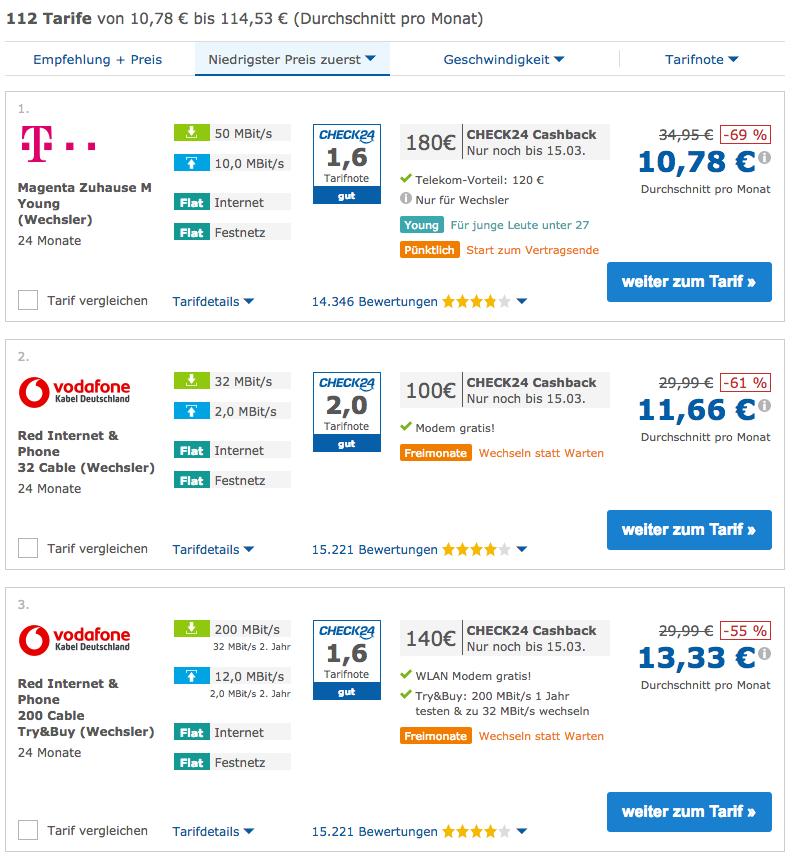
\includegraphics[width=1\textwidth,scale=0.8]{images/ds-sys/check24_2}
	\caption{Check24.de DSL contract comparison result. The contracts can be sorted by domain-specific criterias.}
	\label{img:check24_2}
\end{figure}

The other mentioned sites work similarly. They provide more of a ranking than a comparison.\newline


Another interesting type of websites are Question Answering Portals like \emph{Quora} or \emph{GuteFrage}\footnote{https://quora.com, https://gutefrage.net - all last checked: 12.12.2017}. Although comparisons are not their primary goal, a lot of comparative questions are present on those sites.
On Quora, more than 2.380.000 questions have the phrase \enquote{better than} in their title. If \emph{Ruby} and \emph{Python} are added, 10.100 questions remain.\footnote{Checked via Google on 11th of December. Search phrase: \texttt{"better than" site:quora.com} and \texttt{ruby python "better than" site:quora.com}}
Same is true for the German site GuteFrage, though, the numbers are smaller than on Quora.\footnote{334.000 for \texttt{"besser als" site:gutefrage.net} and 78 for \texttt{ruby python "Besser als" site:gutefrage.net}}\newline

More interestingly are systems which can compare any objects on arbitrary properties. Two examples are \emph{Diffen} and \emph{Versus}\footnote{https://diffen.com, https://versus.com - all last checked: 12.12.2017}.

Versus aggregates freely available data sources like Wikipedia and official statistic reports. For example, the comparison of \enquote{Hamburg vs. Berlin} uses Wikipedia for the number of universities, worldstadiums.com for the availability of sport facilities and the Economist for the Big Mac Index. Presumably, some human processing is involved as the possible comparisons are limited. For instance, a comparison of Hamburg and Darmstadt is not possible as Darmstadt is not available on Versus. Likewise, \enquote{Ruby vs. Python} is not possible, Versus suggests to compare \enquote{Rome vs. Pyongyang} instead. Although Versus shows how many users \enquote{liked} the objects, it does not give a clear statement which one is better. For instance, it is not possible to check automatically whether Hamburg or Berlin is better for a short city trip. The user must search manually all valid properties like the number of museums, theaters, the price of public transport tickets and so on.

Similar to Versus, Diffen aggregates different data sources (see figures \ref{img:diffen} and \ref{img:versus}). All in all, the aggregated information is similar to Versus. The comparison is also tabular. Besides the automatically aggregated data, users can add information on their own. Diffen describes itself as \enquote{inspired by Wikipedia}\footnote{https://www.diffen.com/difference/Diffen:About - Last checked: 11.12.2017}. Diffen does not enforce any restrictions on the objects of comparison, but it faces the same problem as Versus as objects are missing. A comparison between Darmstadt and Hamburg is likewise not possible: all cells for Darmstadt in the table are just empty.

\begin{figure}[h]
	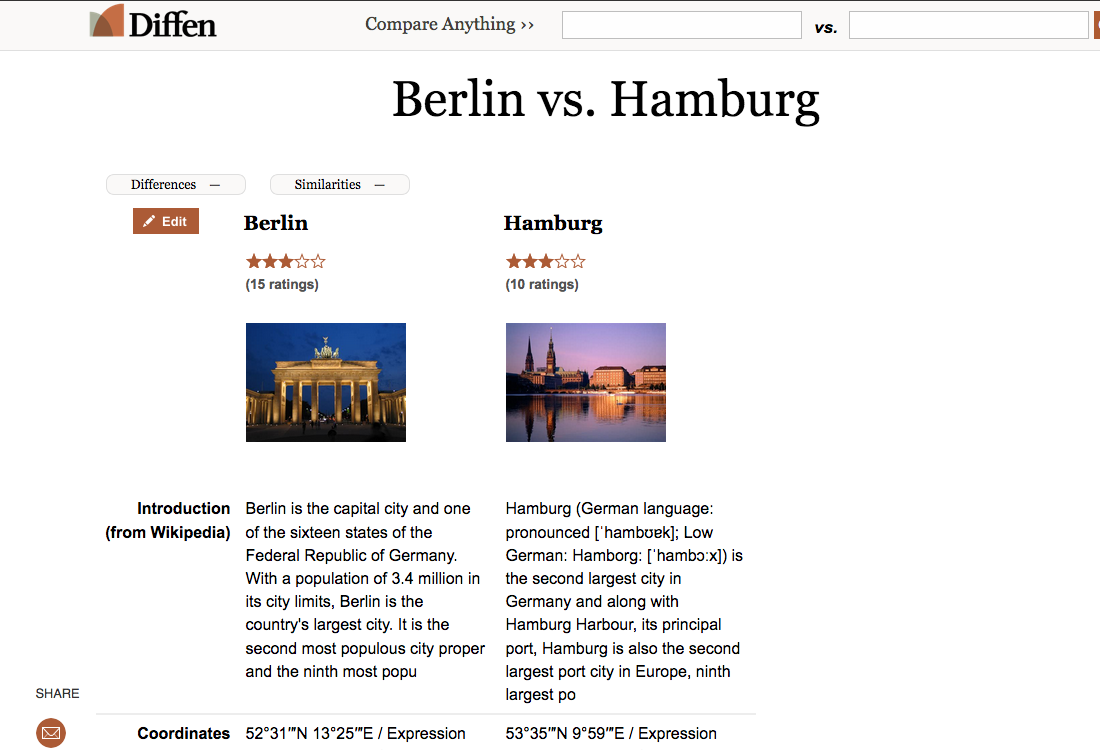
\includegraphics[width=1\textwidth]{images/ds-sys/diffen}
	\label{img:diffen}
	\caption{The comparison of \enquote{Hamburg vs. Berlin} on Diffen.com}
\end{figure}

\begin{figure}[h]
	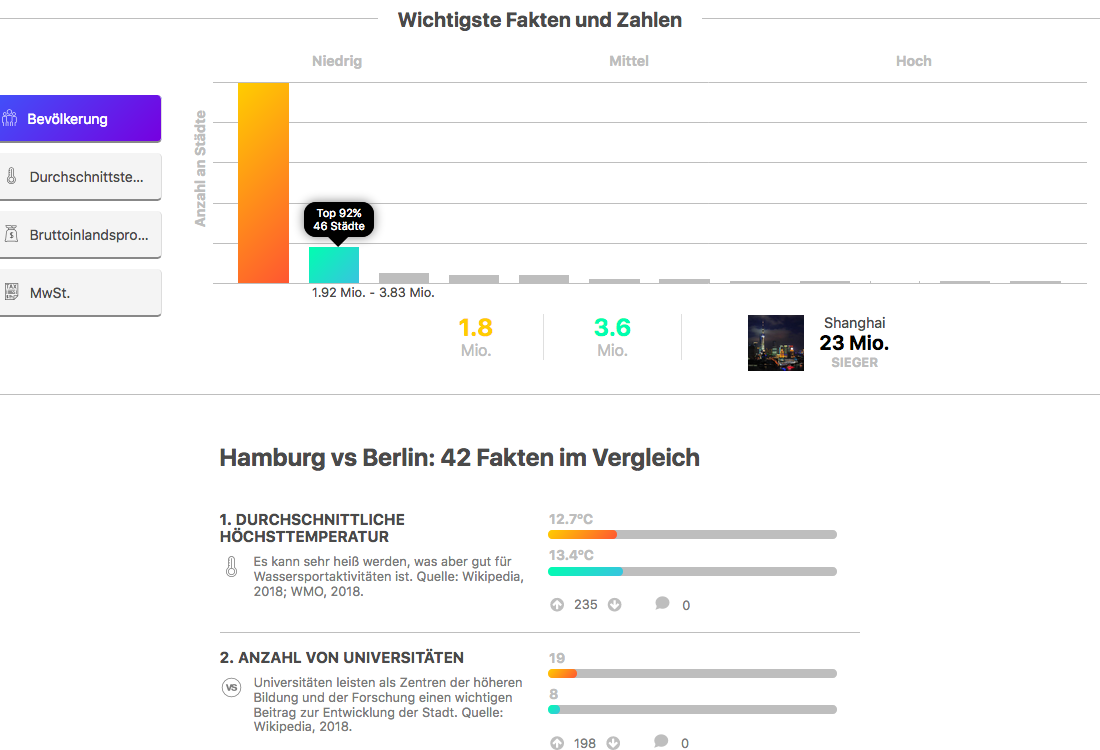
\includegraphics[width=1\textwidth]{images/ds-sys/versus}
	\label{img:versus}
	\caption{The comparison of \enquote{Hamburg vs. Berlin} on Versus.com}
\end{figure}

Neither Versus nor Diffen provides a comprehensible reason why an object is better than another one. They merely aggregate facts and bring them face to face. Despite the aggregation approach of both systems, many meaningful comparisons are not possible or not helpful (like \enquote{Hamburg vs. Darmstadt}, \enquote{Java vs. C\#}, \enquote{Dr Pepper vs. Orange Juice}).
Also, the user can not define the properties for the comparison. The sites provide every information available for the objects. For instance, Versus shows 42 properties for \enquote{Hamburg vs. Berlin} and only 35 for \enquote{Hamburg vs. Munich}.
\newline

To summarize, a lot of different comparison portals exist and are widely used. Especially the domain-specific portals do a good job, but inflexibility dearly buys the performance. First, the portals can only compare objects on predefined properties. Second, the data acquisition is not fully automatic. Domain-unspecific systems are good at aggregating information but do not provide a reasonable explanation to prefer X over Y.

Adding information like comments and product reviews can enrich the comparison with reasons and opinions, such as \enquote{Ruby is easier to learn than C} or \enquote{Python is more suitable for scientific applications than Erlang as many libraries exist}.


\section{Vector Representations for Documents}
The following sections presents methods to transform a document of arbitrary size into a fixed length numeric vector. This vector can than be used as a feature for machine learning. This section is based on \cite{martin2009speech}.

\subsection{Similarity of vectors}

\subsection{n-gram vectors}
An n-gram is a sequence of n words. For instance, all bigrams (n=2) of the previous sentence are: \emph{An n-gram}, \emph{n-gram is}, \emph{is a}, \emph{a sequence}, \emph{sequence of}, \emph{of n}, \emph{n words}. N-grams can be used to generate a fixed-sized vector for every document in a corpus.

For that, all n-grams present in the corpus are extracted into a list. The vector for each document has the size of the n-gram list. The first component of the vector represents the first n-gram in the list and so on. If the document contains the k-th n-gram from the list, the k-th component of the vector is set to one (or to the number of occurence of that n-gram in the document). Otherwise, it is set to zero.

If unigrams (n=1) are used, all sequence information contained in the sentence is lost. This is also called \emph{bag-of-words}.

Instead of using the words of the documents, their \emph{part of speech} can be used to generate n-grams. Parts of speech are for example \emph{nouns}, \emph{verbs} or \emph{personal pronouns}. This can be useful to introduce another layer of abstraction.

\subsection{Term frequency, inverse document frequency}
N-gram vectors as described above ignore the fact that not all words (or n-grams) in a document are equally important. For example, articles or the word \enquote{\emph{to}} are present in almost every English document. In general, they only contribute little to the meaning of the sentence.\footnote{Extremly frequent words (called \emph{stopwords}) are often removed from the documents as a preprocessing step.}

To support the importance of a n-gram, weighted values can be used instead of the number of occurences of n-grams as the vector's components. Frequent n-grams in the corpus get a value near zero, while seldom n-grams get a value near one. A common weighting factor is \emph{term frequency, inverse document frequency (tf-idf)}.

\begin{equation*}
\begin{multlined}
\text{tf}(t) = \frac{\text{number of times t appears the document}}{\text{total number of terms in the document}} \\
\hfill\\
\text{idf}(t) = \frac{\text{total number of documents in the corpus}}{\text{number of documents containing t}} \\
\hfill\\
\text{tf-idf(t)} = \text{tf}(t) \times \log (\text{idf}(t)) \\
\end{multlined}
\end{equation*}



\subsection{Mean Word Embeddings}
The vector representations presented above produce \emph{sparse} and long vectors. For example, a corpus of short messages might contain six-thousand n-grams, but every message only contains about sixty n-grams. This will create vectors with 99\% zeros. However, a machine learning algorithm has to learn six-thousand parameters. Short and \emph{dense vectors} (for example, 300 components) reduce the number of learnable parameters.

A popular method for creating dense vectors for \emph{words} (called \emph{word embeddings}) is \emph{word2vec} (\cite{NIPS2013_5021}). Word2Vec learns a word embedding for the word \emph{w} by training a neural network to predict words preceding \emph{w}.


\subsection{Sentence Embeddings}